\documentclass[10pt,a4paper]{article}
\usepackage[margin=2.2cm]{geometry}
\usepackage{amsmath,amssymb}
\usepackage{graphicx}
\usepackage{booktabs,tabularx,longtable,array}
\usepackage[font=small,labelfont=bf]{caption}
\usepackage{xcolor}
\usepackage{enumitem}
\usepackage{microtype}
\usepackage{tikz}
\usetikzlibrary{arrows.meta,positioning,fit,calc}
\usepackage[colorlinks=true,linkcolor=blue!50!black,citecolor=blue!50!black,urlcolor=blue!50!black]{hyperref}

\setlist{itemsep=1pt,topsep=3pt}
\renewcommand{\topfraction}{0.9}
\renewcommand{\bottomfraction}{0.8}
\renewcommand{\textfraction}{0.07}
\renewcommand{\floatpagefraction}{0.85}
\setcounter{totalnumber}{4}
\newcolumntype{L}{>{\raggedright\arraybackslash}X}
\newcommand{\code}[1]{\texttt{\small #1}}
\newcommand{\vmax}{v_{\max}}
\newcommand{\vmin}{v_{\min}}
\graphicspath{{figures/}{../results/}}
\newcommand{\est}{\textcolor{gray!75!black}{\textbf{Established}}}
\newcommand{\adp}{\textcolor{orange!80!black}{\textbf{Adapted}}}
\newcommand{\new}{\textcolor{green!45!black}{\textbf{New}}}

\title{\textbf{ECG and Doppler envelopes from ultrasound DICOM images}\\[2pt]
\large Methods summary for \code{dicom2waveform\_standalone.py}}
\date{13 October 2026}

\begin{document}
\maketitle

\begin{center}
\fbox{\parbox{0.9\linewidth}{\small \textbf{Internal use.} Figures~\ref{fig:pw}--\ref{fig:alias} and~\ref{fig:params}
show crops of clinical images (Doppler strip and ECG only, no header area), relabelled as Examples 1--5.
Do not distribute outside the institution. Figure~\ref{fig:dp} is synthetic.}}
\end{center}

\section*{Summary}
\begin{itemize}
\item \textbf{Problem.} Spectral Doppler (PW, CW) and tissue Doppler (TDI) DICOMs store the scanner's
\emph{rendered display}, not the Doppler signal. The ECG exists only as burned-in pixels. The timing between
ECG and Doppler events (for example R-peak $\to$ aortic valve closure) has to be recovered from the picture.
\item \textbf{Outputs.} On one time axis: the ECG, the outer velocity envelopes $\vmax$ and $\vmin$, mean
velocities, R-peaks, valve clicks and aortic valve closure (AVC), plus quality flags (modality, aliasing, SNR proxy).
\item \textbf{Method.} The header gives the calibration. The display is cleaned (overlays, text, sweep), and the
envelope is a globally optimal smooth curve, found by dynamic programming (DP) on a noise-referenced
signal-density image. PW/TDI aliasing is detected and unwrapped automatically.
\item \textbf{Accuracy.} Against the scanner's own envelope trace (5 vascular images): mean absolute error
\textbf{1.9~cm/s} (held-out 2.2~cm/s, $r=0.99$). This is the best of all candidate methods tested; the next best had 3.7~cm/s and the
spectrum methods 8--45~cm/s. R-peaks were found in all 44 cardiac test images. On an external cardiac dataset (EchoXFlow, GE,
126 clinician-drawn envelopes) the error is 9\,\% (PW) and 7\,\% (CW) of the peak velocity, with shape correlation 0.97--0.98.
\item \textbf{What is new.} Most building blocks are established: header calibration, overlay masking, ECG-by-colour, noise-referenced
thresholds, Pan--Tompkins R-peaks, DP with an L1 smoothness prior, and click detection. As far as a literature search (October 2026) could
establish, these parts are new: (i) a globally optimal DP for the Doppler maximum-velocity envelope, (ii) its outer-edge cost with a free
interior, (iii) density normalisation so that one setting serves PW, CW and TDI, (iv) the smoothness prior expressed as a physical acceleration, and
(v) post-hoc, per-column aliasing unwrapping on the rendered display (Section~\ref{sec:novelty}).
\item \textbf{State of the art?} Partly. Head-to-head with the only public learned model (EchoNet-Measurements) on 258 EchoXFlow
measurements, DP read at the marked beats is as accurate or better for e$'$, A, LVOT and AV peaks (significantly for AV), and
worse for TR Vmax, where clinicians measure in the faint tail of the jet (Section~\ref{sec:external}). DP still needs per-beat
peak picking to be fully automatic.
\item \textbf{Main limitations.} The edge convention depends on the measurement and the reader: our user marks CW jets at the dense
edge (DP $\sim$15~cm/s outside), GE clinicians mark TR Vmax in the faint tail (DP $\sim$77~cm/s inside) and e$'$ $\sim$2~cm/s inside
the outer edge. One global setting cannot match all; per-measurement settings are needed. Mirror artefacts are traced as flow.
\end{itemize}

\tableofcontents

%=====================================================================================
\section{The problem}

\subsection{What the DICOM contains}
Each file is a single frame. It shows the B-mode image at the top, the ECG along the lower edge of the B-mode
area, and the scrolling spectral display below it (Figure~\ref{fig:pipeline}). For the spectral display, the
DICOM \emph{Ultrasound Region Calibration} module gives the pixel box, the time per column ($\Delta t$, 2.6--3.5~ms),
the velocity per row ($\Delta v$) and the zero-velocity row. The pixels themselves are a rendering:
\begin{itemize}
\item \textbf{Log-compressed grey levels} (or a colour map for TDI). Gain, dynamic range and reject settings
are unknown, so grey levels are only a monotonic proxy of Doppler power.
\item \textbf{Overlays} drawn on top: the baseline, time markers, the ECG trace, scale ticks, text, and sometimes a
vendor envelope trace.
\item \textbf{A circular buffer}: the display is written left to right and wraps around. The write position
(the \emph{sweep}) holds no data. The oldest sample sits just right of it.
\item \textbf{Display artefacts}: wall-filter clutter near the baseline, mirror images of strong flow on the
opposite side, valve clicks (saturated vertical lines), speckle, and \emph{aliasing} in PW/TDI (flow
faster than the display limit re-enters at the opposite limit).
\item \textbf{Different spectrum shapes}: CW spectra are filled from the baseline, PW spectra can be hollow
(spectral window), and TDI shows thin bands in a colour map.
\item \textbf{No calibrated ECG}: the trace has no amplitude scale, and the scanner clips tall R-waves to its display box.
\end{itemize}

\subsection{Required outputs}
\begin{center}\small
\begin{tabularx}{\linewidth}{@{}lL@{}}
\toprule
Output & Definition \\ \midrule
\code{t} & time (s), oldest sample first (sweep removed by rotation; NaN = no data) \\
\code{ecg} & ECG traced from the pixels, arbitrary units, isoelectric $\approx0$, $\max|\cdot|=1$ \\
\code{v\_max}, \code{v\_min} & outer edge of the positive / negative spectrum (cm/s; 0 when no flow on that side) \\
\code{v\_mean}, \code{v\_mean\_pos}, \code{v\_mean\_neg} & intensity-weighted mean velocity inside the detected
flow region: both halves (signed), positive half, negative half \\
\code{t\_rpeaks}, \code{t\_clicks}, \code{t\_avc} & R-peaks, valve clicks, aortic valve closure (s) \\
\code{conf\_pos}, \code{conf\_neg} & per-column confidence of the envelope (0--1) \\
\code{flags} & modality (PW/CW/TDI), ECG found/clipped, aliasing suspected/corrected, number of clicks, SNR proxy \\
\bottomrule
\end{tabularx}
\end{center}
Velocities carry the sign given by the DICOM header (\code{PhysicalDeltaY}). If the operator inverted the
display, this sign is opposite to the on-screen label.

\subsection{Data used for development and validation}
\begin{center}\small
\begin{tabularx}{\linewidth}{@{}lrLL@{}}
\toprule
Set & $n$ & Content & Reference \\ \midrule
Vascular, vendor trace & 5 & Philips iU22, PW & scanner's own envelope trace (only pixel-accurate real reference) \\
Cardiac & 44 & Philips iE33 / EPIQ CVx / Affiniti 70C; PW, CW, TDI & manual peak/timing marks on 17; DICOM heart rate on 11 \\
Synthetic & 224 & rendered displays (PW, CW, TDI, aliasing) at $-3$ to 30~dB & known truth (dev / held-out split) \\
\bottomrule
\end{tabularx}
\end{center}

%=====================================================================================
\section{Processing pipeline}
Figure~\ref{fig:pipeline} shows the stages of the standalone script. The DP envelope is described in
Section~\ref{sec:dp}, and the other components in Section~\ref{sec:components}. A typical image
(1024$\times$768) takes $\sim$0.2~s.

\begin{figure}[h]
\centering
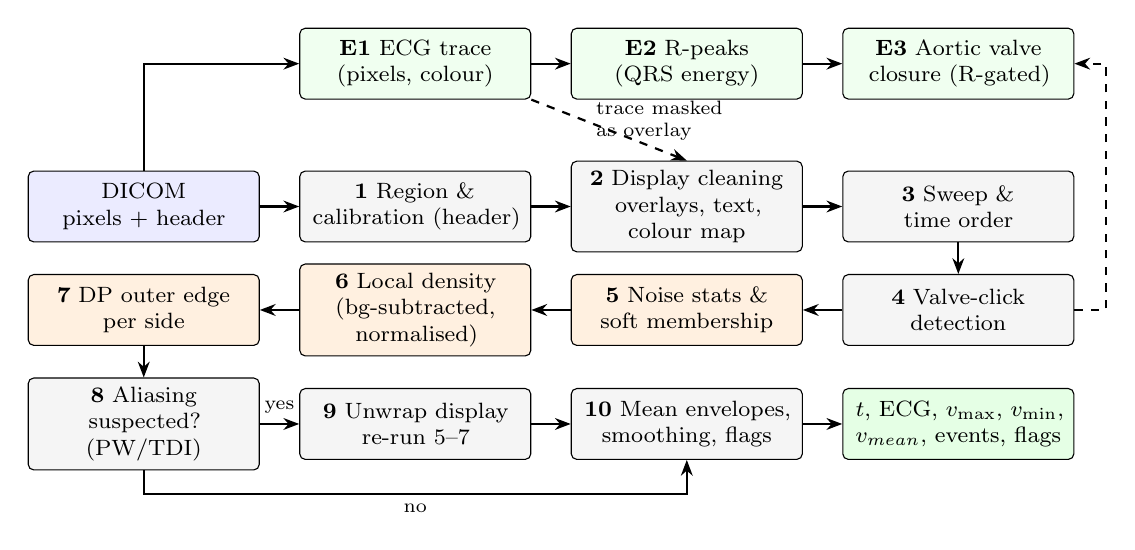
\begin{tikzpicture}[
  box/.style={draw, rounded corners=2pt, align=center, font=\footnotesize, minimum height=9mm, text width=27mm, fill=#1},
  box/.default=gray!8,
  arr/.style={-{Stealth[length=2mm]}, thick},
  node distance=4mm and 5mm]
\node[box=blue!8] (dcm) {DICOM\\pixels + header};
\node[box, right=of dcm] (cal) {\textbf{1} Region \&\\calibration (header)};
\node[box, right=of cal] (clean) {\textbf{2} Display cleaning\\overlays, text, colour map};
\node[box, right=of clean] (sweep) {\textbf{3} Sweep \&\\time order};
\node[box, below=of sweep] (click) {\textbf{4} Valve-click\\detection};
\node[box=orange!12, left=of click] (memb) {\textbf{5} Noise stats \&\\soft membership};
\node[box=orange!12, left=of memb] (dens) {\textbf{6} Local density\\(bg-subtracted, normalised)};
\node[box=orange!12, left=of dens] (dp) {\textbf{7} DP outer edge\\per side};
\node[box, below=of dp] (alias) {\textbf{8} Aliasing\\suspected? (PW/TDI)};
\node[box, right=of alias] (unwrap) {\textbf{9} Unwrap display\\re-run 5--7};
\node[box, right=of unwrap] (mean) {\textbf{10} Mean envelopes,\\smoothing, flags};
\node[box=green!10, right=of mean] (out) {$t$, ECG, $\vmax$, $\vmin$,\\$v_{mean}$, events, flags};
\node[box=green!6, above=9mm of cal] (ecg) {\textbf{E1} ECG trace\\(pixels, colour)};
\node[box=green!6, right=of ecg] (rpk) {\textbf{E2} R-peaks\\(QRS energy)};
\node[box=green!6, right=of rpk] (avc) {\textbf{E3} Aortic valve\\closure (R-gated)};
\draw[arr] (dcm) -- (cal); \draw[arr] (cal) -- (clean); \draw[arr] (clean) -- (sweep);
\draw[arr] (sweep) -- (click); \draw[arr] (click) -- (memb); \draw[arr] (memb) -- (dens); \draw[arr] (dens) -- (dp);
\draw[arr] (dp) -- (alias); \draw[arr] (alias) -- node[above, font=\scriptsize]{yes} (unwrap);
\draw[arr] (unwrap) -- (mean); \draw[arr] (alias.south) -- ++(0,-3mm) -| node[pos=0.25, below, font=\scriptsize]{no} (mean.south);
\draw[arr] (mean) -- (out);
\draw[arr] (dcm.north) |- (ecg.west);
\draw[arr] (ecg) -- (rpk); \draw[arr] (rpk) -- (avc);
\draw[arr, dashed] (ecg.south east) -- node[right, font=\scriptsize, align=left, pos=0.35]{trace masked\\as overlay} (clean.north);
\draw[arr, dashed] (click.east) -- ++(4mm,0) |- (avc.east);
\end{tikzpicture}
\caption{Pipeline of \code{extract\_waveforms()}. Orange: the envelope estimator (Section~\ref{sec:dp}).
Green: the ECG branch. The ECG trace is masked out of the Doppler region before the envelope is estimated, and
the click strengths feed the R-gated AVC detector.}
\label{fig:pipeline}
\end{figure}

%=====================================================================================
\section{Candidate envelope methods}
\label{sec:candidates}
Ten envelope estimators were implemented in Python and compared on the same front end (stages 1--4 and 8--9, so all methods
see the same cleaned display); the earlier MATLAB methods are listed for reference. \emph{Spectrum methods} treat every column as a power spectrum on its own. Because only the display
is available, they are image-domain adaptations: the grey level is de-compressed with an assumed 40~dB dynamic
range, and each side needs a flow-presence gate, since the published methods assume the flow direction is known.
\emph{Image methods} use the 2-D picture. Table~\ref{tab:candidates} summarises them, and Figure~\ref{fig:bench}
shows the two main comparisons.

\begin{table}[!htbp]
\centering\footnotesize
\caption{Candidate envelope methods. Vendor MAE: mean absolute error against the scanner's envelope trace
(5 vascular images, cm/s). Synthetic: median error on the held-out synthetic split, in \% of the display span.
IPS = integrated power spectrum (cumulative power along the column).}
\label{tab:candidates}
\setlength{\tabcolsep}{4pt}
\begin{tabularx}{\linewidth}{@{}>{\raggedright\arraybackslash}p{2.4cm}LLrr@{}}
\toprule
Method & Principle & Main limitations & Vendor & Synth. \\ \midrule
\multicolumn{5}{@{}l}{\textit{Image methods}} \\
Fixed threshold & outermost pixel above a fixed grey level & gain-dependent; speckle and text beyond the
edge are taken as flow; failed completely on one image (41~cm/s) & 11.8 & 3.2\% \\
Otsu + morphology & Otsu threshold, closing/opening/filling, outermost pixel & threshold too high on clean
displays (cuts the faint fringe); breaks down on sparse TDI at low SNR (22\%) & 3.68 & 1.7\% \\
OMM (Latham 2021) \cite{latham} & Otsu with EM-selected windows, hierarchical morphology, largest-gap rule &
designed for STFTs of the audio signal (emulated here); reads under the edge & 4.67 & 1.6\% \\
MATLAB legacy (curvature, cumulative intensity) & per-column threshold on curvature or cumulative intensity, median filter &
gain-dependent; tracks the bright core, under-reads; jittery & 18.1 & -- \\
MATLAB DP (two-region split) & DP on a cost that splits each column into flow / no flow &
assumes a spectrum filled from the baseline; collapses on hollow PW and TDI spectra & 2.23 & 4.1\%$^\dagger$ \\
\textbf{DP (this work)} & soft membership $\to$ density $\to$ DP outer edge with acceleration prior &
edge level calibrated on vascular PW only (see Section~\ref{sec:limits}); mirror bands are traced as flow & \textbf{1.92} & \textbf{1.2\%} \\
\midrule
\multicolumn{5}{@{}l}{\textit{Spectrum methods (per column, on the de-compressed display)}} \\
Percentile \cite{marasek} & velocity at 95\% of the IPS & depends on the noise power in the column;
overshoots at low SNR & 10.1 & 10.4\% \\
GM \cite{marasek} & knee of the IPS: farthest point from the line from the peak-power point to the IPS end & sensitive to
noise slope and clutter & 8.46 & 5.1\% \\
MGM \cite{moraes} & as GM, line from the first to the last IPS point & as GM & 11.4 & 4.5\% \\
SNSI \cite{steinman} & intersection of the signal and noise slopes of the IPS & needs a clean noise region in each column & 17.9 & 5.4\% \\
Adaptive SNSI \cite{kathpalia} & SNSI or altered GM, chosen per column, with an adaptive power threshold &
best spectrum method, but still column-wise jitter; manual baseline shift for aliasing & 13.3 & 3.1\% \\
QIA \cite{li} & quadratic iteration on the IPS curve & unstable on rendered displays & 44.8 & 5.8\% \\
\bottomrule
\end{tabularx}

\smallskip\raggedright $^\dagger$all seeds (ablation). MATLAB legacy methods: MATLAB implementation, vendor MAE as reported there.
MATLAB DP: 2.31~cm/s in MATLAB, 2.23~cm/s as Python port.
\end{table}

\begin{figure}[!htbp]
\centering
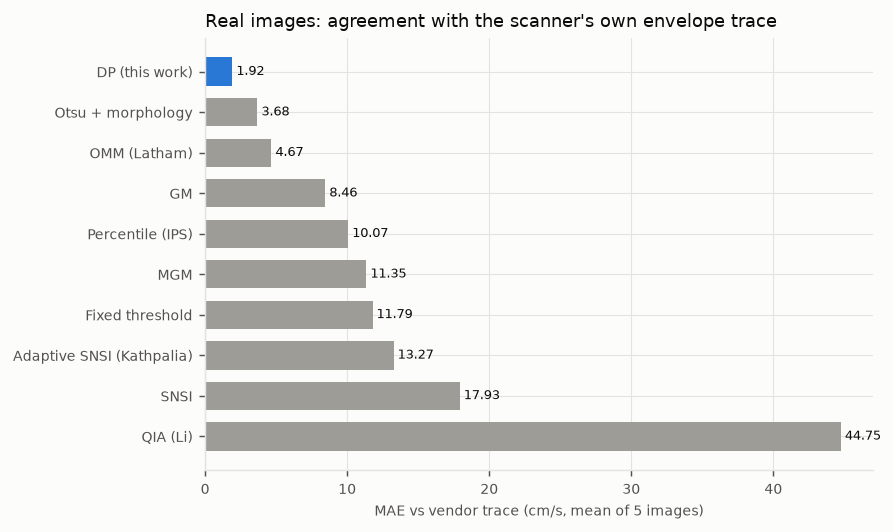
\includegraphics[width=0.62\linewidth]{fig_vendor.png}\\[4pt]
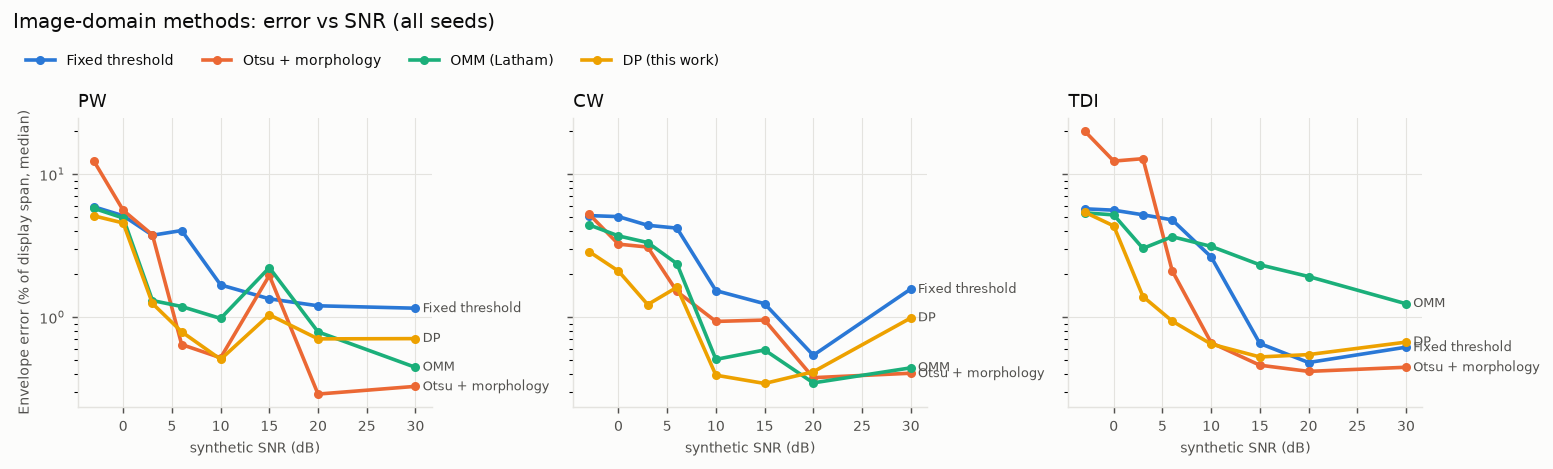
\includegraphics[width=\linewidth]{fig_snr_image.png}
\caption{Top: agreement with the scanner's own envelope trace (5 vascular images). Bottom: error against
synthetic truth as a function of SNR for the image methods (spectrum methods are worse; see the benchmark report).
The real images have SNR proxies of 15--43~dB, at or above the synthetic 20--30~dB range. On real data, rendering
effects (clutter, mirror bands, clicks, text) separate the methods more than noise does.}
\label{fig:bench}
\end{figure}

\paragraph{Why DP.} The DP method is the most accurate on the real reference and on synthetic data, and it
degrades most gracefully at low SNR. On synthetic data at $\le$3~dB the error falls as more 2-D information is used:
column-wise 8.6\%, with 1-D smoothing 6.4\%, 2-D segmentation 5.1\%, DP 2.8\%. The same parameter set works for
spectral Doppler and TDI. At high SNR, Otsu and OMM are equivalent on synthetic data. They lose on the real
images because a single global threshold does not fit both the dense core and the faint fringe of the spectrum.

\paragraph{Published approaches not benchmarked here.} The literature search (Section~\ref{sec:novelty}) found further envelope tracers
that were not implemented, because no code is available or they need training data:
\begin{itemize}
\item \textbf{Objective threshold + biggest gap} on screen captures \cite{zolgharni}: a histogram-gradient threshold, removal of small clusters,
and the outermost pixel above the largest gap per column. It was validated against three experts (peak velocity $R^2=0.98$). Like Otsu/OMM it is
a single global threshold with per-column extraction, so it has the same weakness on faint fringes.
\item \textbf{Kalman tracking with a statistical shape model} \cite{wang2008}: recursive (causal) estimation. It has no global optimum and needs a trained shape model.
\item \textbf{Edge-following with physiological constraints} on transcranial Doppler \cite{tcd2020}: several binary segmentations, keeping the best-scoring envelope.
\item \textbf{Active contour (GVF snake) after k-means clustering} \cite{zamzmi}: a global smooth curve, but it needs initialisation and has no
guaranteed optimum.
\item \textbf{Learned models}: U-Net envelope segmentation for mitral inflow \cite{mitralunet}, multi-beat TDI networks \cite{lane2023}, and
EchoNet-Measurements \cite{echonetmeas}, which gives peak velocities only. These need labelled training data, generalise only as far as their
training vendors and views, and (except EchoNet-Measurements, compared in Section~\ref{sec:external}) have no public weights
(Section~\ref{sec:public}).
\end{itemize}

%=====================================================================================
\section{The dynamic-programming envelope}
\label{sec:dp}
The envelope is the outer boundary of the flow region. It is estimated separately for the positive and the negative
side of the baseline. Each side is re-indexed outward from the baseline: row $k=0$ is zero velocity, and $|v| = k\,|\Delta v|$.
The idea: turn the display into a map of \emph{local signal density}, then find the single smooth curve per side
that best separates ``signal outside the edge'' from ``no signal just inside it'' over the whole recording at once.
Figure~\ref{fig:dp} shows the steps on a synthetic image with known truth.

\begin{figure}[!htbp]
\centering
\includegraphics[width=\linewidth]{dp_steps.pdf}
\caption{DP envelope on a synthetic PW display (10~dB, wall clutter, speckle; no patient data).
(b) Soft membership highlights the flow but also scattered noise. (c) The background-subtracted, normalised local density
suppresses the noise, and the DP edges (red/cyan) follow the true edges (dashed white); mean error 1.0~cm/s.
(d) One column: density profile, edge cost $C(k)$ and the chosen edge. The edge lies where the density falls through
$\theta$, and the isolated noise blob near 80~cm/s is not enough to move it.}
\label{fig:dp}
\end{figure}

\subsection{Step 1: noise-referenced soft membership}
Let $L$ be the cleaned display level (0--255). From all valid pixels the script estimates the noise level
$\mu=\mathrm{median}(L)$ and its spread $\sigma = 1.4826\,\mathrm{MAD}(L)$, plus Otsu's threshold $T_{\mathrm{Otsu}}$ \cite{otsu}.
The signal threshold and the top of the noise are
\begin{equation}
T = \min\!\big(\mu + \max(\Delta_n, k_\sigma\sigma),\; T_{\mathrm{Otsu}}\big), \qquad n_0 = \mu + s\,\max(\sigma,1),
\end{equation}
and every pixel gets a membership that ramps linearly from noise to signal:
\begin{equation}
m = \mathrm{clip}\!\left(\frac{L-n_0}{\max(T-n_0,1)},\,0,\,1\right).
\end{equation}
The noise margin keeps the faint outer fringe on clean displays, and the Otsu cap keeps the threshold sensible on
very dense displays, where median and MAD no longer describe the noise. Because gain acts roughly as an additive offset on a
log display, referencing the threshold to the measured noise makes it gain-invariant. Soft rather than binary membership
made faint flow count partially instead of being cut off; this was the key refinement of the original MATLAB DP.

\subsection{Step 2: local density, background subtraction and normalisation}
Membership is averaged over a small window ($9\times5$ pixels, rows $\times$ columns), which gives a local density
$\tilde d$: evidence that a pixel lies inside the flow region rather than on an isolated noise speck. Two corrections follow:
\begin{align}
d' &= \mathrm{clip}\!\left(\frac{\tilde d - b}{1-b},0,1\right), \quad b = P_{50}(\tilde d) && \text{(noise background, if $b<0.9$)}\\
d &= \mathrm{clip}\!\left(\frac{d'}{\max(P_{99}(d'),\,f)},0,1\right) && \text{(typical in-flow density $\to$ 1)}
\end{align}
Without background subtraction, uniform noise rewards moving the edge outward, and the edge runs to the display limit at
low SNR. Normalisation makes the edge level $\theta$ mean ``a fraction of this image's typical in-flow density''.
That lets one setting serve dense renderings (vascular, CW) and sparse ones (speckled TDI). On TDI only, each side is also
normalised by its running column maximum over $\pm10$~ms (floor 0.15), so faint low-velocity tissue
segments are not dropped.

\subsection{Step 3: the outer-edge cost}
For column $x$ and candidate edge $k$:
\begin{equation}
C_x(k) = \underbrace{\sum_{j>k} (d_j-\theta)_+}_{\text{signal left outside}}
\;+\; \underbrace{\sum_{k-h<j\le k} w_j\,(\theta-d_j)_+}_{\text{no signal just inside}}
\;+\; \underbrace{\rho\,k}_{\text{weak prior: no flow}},
\end{equation}
with $(\cdot)_+=\max(\cdot,0)$, $h$ the inner band (5\% of the display height), and $w_j=0.01$ inside the wall-filter
band next to the baseline (3\% of the height), $w_j=1$ elsewhere. Only the band just inside the edge has to hold
signal; the interior deeper than $h$ is free. This handles hollow PW spectra and thin TDI bands, where the
original MATLAB two-region split (``everything between baseline and edge is flow'') collapsed to $v=0$. On pure noise
($d<\theta$ everywhere) the minimum is $k=0$: no flow. An edge that ends inside the wall band is reported as 0.

\subsection{Step 4: smoothness prior and the global solution}
The edge path $e_1,\dots,e_W$ of each side minimises
\begin{equation}
E(e) = \sum_x C_x(e_x) + \lambda \sum_{x} |e_x - e_{x-1}|, \qquad
\lambda = \frac{|\Delta v|/\Delta t}{a_{\mathrm{ref}}}, \quad
a_{\mathrm{ref}} = a_0\,\frac{V_{\mathrm{display}}}{100~\mathrm{cm/s}}.
\end{equation}
Moving the edge by one row between neighbouring columns means an acceleration of $|\Delta v|/\Delta t$. So the L1 term is a
\emph{physiological acceleration prior}: at acceleration $a_{\mathrm{ref}}$, moving the edge costs as much as one
misclassified pixel. It is expressed in physical units, so it means the same on every image (pixel sizes differ $\sim$30$\times$ in
velocity between TDI and CW). Scaling with the display range $V_{\mathrm{display}}$ (largest |velocity| shown) prevents clipping of steep
systolic upstrokes on high-range displays. The L1 form allows abrupt valve-opening onsets, which a quadratic penalty would round off.

The minimum is found exactly by dynamic programming:
$F_x(k) = C_x(k) + \min_j \big[F_{x-1}(j) + \lambda|k-j|\big]$, followed by backtracking. The inner minimum is an L1
distance transform \cite{felzenszwalb}, computed in $O(D)$ per column with a forward and a backward running minimum. The whole
image therefore costs $O(D\,W)$ (a few ms per side). Transitions across the sweep are free, because the columns on either side are not
adjacent in time. A per-column confidence, $(\overline{C_x} - C_x(e_x)) / (\max_k C_x - \min_k C_x)$, is returned as
\code{conf\_pos}/\code{conf\_neg}. Finally $\vmax = e^{\mathrm{pos}}|\Delta v|$ and $\vmin = -e^{\mathrm{neg}}|\Delta v|$.

\subsection{DP parameters}
Table~\ref{tab:dpparams} lists the parameters of the envelope. Only $\theta$ and the density normalisation were fitted to data:
$\theta$ by leave-one-image-out on the vendor traces (0.5 chosen in 3 of 5 folds), and the normalisation on the synthetic dev split.
The rest are physically motivated defaults. Figure~\ref{fig:params} shows the effect of the two most important ones.

\begin{table}[!htbp]
\centering\small
\caption{Envelope parameters (YAML sections \code{likelihood} and \code{dp}). All parameters, including those of the other
components, are documented in \code{dicom2waveform\_config.yaml}.}
\label{tab:dpparams}
\setlength{\tabcolsep}{4pt}
\begin{tabularx}{\linewidth}{@{}>{\raggedright\arraybackslash}p{4.4cm}>{\raggedright\arraybackslash}p{1.5cm}LL@{}}
\toprule
Key & Default & Meaning & Effect of increasing \\ \midrule
\multicolumn{4}{@{}l}{\textit{section} \code{dp:}} \\
\code{edge\_density} ($\theta$) & 0.5 & density level at which the edge is placed & edge moves inward (less faint fringe) \\
\code{edge\_density\_tdi} & null & separate $\theta$ for TDI (null = same) & -- \\
\code{reference\_accel\_cm\_s2} ($a_0$) & 640 & acceleration at which moving the edge costs one pixel & less smoothing; follows narrow spikes \\
\code{accel\_scale\_with\_range}, \code{reference\_range\_cm\_s} & true, 100~cm/s & scale $a_0$ with the display range & -- \\
\code{inner\_band\_rel} ($h$) & 0.05 & band inside the edge that must hold signal (fraction of height) & ignores thinner bands / gaps \\
\code{height\_prior} ($\rho$) & 0.01 & cost per row of edge height & weak flow more often reported as 0 \\
\code{wall\_band\_rel} & 0.03 & wall-filter band near the baseline (fraction of height) & more low-velocity signal treated as clutter \\
\code{background\_percentile} & 50 & density percentile subtracted as noise & more aggressive noise removal \\
\code{normalise\_percentile}, \code{normalise\_floor} & 99, 0.1 & density mapped to 1 (typical in-flow) & -- \\
\code{local\_norm\_s}, \code{\_floor}, \code{\_modalities} & 0.01~s, 0.15, [TDI] & per-column local normalisation & keeps fainter segments \\
\midrule
\multicolumn{4}{@{}l}{\textit{section} \code{likelihood:}} \\
\code{noise\_margin} ($\Delta_n$) & 32 & signal threshold above the noise median (grey levels) & less faint signal counted \\
\code{noise\_spread\_factor} ($k_\sigma$) & 4 & same, in robust SDs of the noise & as above \\
\code{soft\_low\_factor} ($s$) & 1.5 & membership starts rising $s\sigma$ above the noise & -- \\
\code{density\_window\_px\_rows}, \code{\_cols} & 9, 5 & density window in px (or \code{\_cm\_s}, \code{\_s} if $>0$) & smoother; cuts narrow peak tips \\
\bottomrule
\end{tabularx}
\end{table}

\begin{figure}[!htbp]
\centering
\includegraphics[width=\linewidth]{params.pdf}
\caption{Effect of the main DP parameters on one beat of Example 1 (PW, $\vmax$ only). (a) Lowering $\theta$ moves the edge
outward onto the faint fringe and picks up isolated bright specks; raising it pulls the edge in. (b) A low $a_{\mathrm{ref}}$
smooths the curve and flattens narrow spikes; a high one follows them.}
\label{fig:params}
\end{figure}

%=====================================================================================
\section{Other components of the script}
\label{sec:components}

\subsection{Region, calibration and display cleaning (stages 1--3)}
\begin{itemize}
\item \textbf{Region by unit codes}: the spectral region is the one with seconds horizontally and cm/s vertically, and the B-mode region the one with
cm on both axes. Regions are never chosen by their order in the header, which varies between files.
\item \textbf{Zero-velocity row} = header \code{ReferencePixelY0}. The header wins over pixel detection, which
can lock onto dense saturated flow. A mismatch with the drawn baseline is reported as a warning. Both signs of
\code{PhysicalDeltaY} are handled; a positive sign (inverted display) is routine in vascular imaging.
\item \textbf{Overlays are masked, not zeroed}: the drawn baseline (and its colour, which is also used for time markers), chromatic pixels on
grey displays (ECG, markers, vendor traces), grey pixels on colour-map displays (text, ticks), and white text: small
bright components with a dark surround (saturated flow has a bright surround). Masked pixels are filled by vertical
interpolation.
\item \textbf{Colour map}: TDI copper maps are converted to a level by luminance $\times 255/160$.
\item \textbf{Sweep and time order}: columns without the drawn baseline (runs $\ge3$~px) are the sweep. They are set to NaN and
never interpolated. All outputs are rotated so time runs oldest $\to$ newest.
\item \textbf{Modality}: CW from the region data type, TDI from the colour map or a display range below 40~cm/s, PW otherwise.
\end{itemize}

\subsection{ECG and R-peaks (E1, E2)}
The ECG trace is found in a band of rows around the lower edge of the B-mode region: it is the colour that covers most
columns without being a horizontal line, and the baseline colour is excluded explicitly. Small components are dropped.
In each column the sample is taken at the stroke top or bottom at local extremes (so R and S keep their full amplitude),
and at the stroke centre elsewhere. Gaps up to 50~ms are interpolated, but never across the sweep. Flat runs at the extreme row raise the
\code{ecg\_clipped} flag. The trace is then masked out of the Doppler region.

R-peaks (a port of the earlier MATLAB detector, Pan--Tompkins style \cite{pantompkins}) are detected on \emph{QRS-band energy}: a
zero-phase 8--30~Hz band-pass, squared in robust SD units and smoothed over 100~ms. Using energy rather than amplitude stops tall T-waves
from being counted (they had doubled the heart rate in an earlier version). Peaks need a 250~ms refractory period and at least
0.35$\times$ the upper-half median of the candidate energies; strips hold only 2--8 beats. In RR gaps longer than 1.66$\times$ the expected RR
(from the DICOM \code{HeartRate} tag when present), a search-back adds the most plausible missed beat. An RR-relative T-wave guard
removes small peaks at 20--55\% of RR. Each peak is refined to the largest deflection within $\pm40$~ms. Premature beats are kept on purpose,
because the valve still opens and closes.

\subsection{Valve clicks and aortic valve closure (stage 4, E3)}
Valve clicks are short, broadband, saturated vertical lines (the leaflets, not blood flow). The script takes the column-mean level and
applies a white top-hat with a 35~ms flat window. This removes features narrower than a click but keeps steps such as flow onset, so a
click on the flank of a jet still stands out. Columns more than 12 robust SDs high, in runs no wider than 35~ms, are clicks
(\code{t\_clicks}). The \code{click\_mode} setting controls what the envelope does with them:
\code{keep} (default; trace the display as shown), \code{bridge} (interpolate over them on PW/CW), \code{follow} (the DP may jump to them at no cost),
or \code{off}.

\textbf{AVC} is the strongest click transient 0.20--0.50~s after each R-peak. It needs at least 6 robust SDs (lower than the general
threshold, which is safe because of the R-gating), must lie at least 12~ms from the window edges, and is timed at the half-maximum centroid.
Images without clicks correctly return no AVC.

\subsection{Aliasing detection and correction (stages 8--9)}
A PW spectrum is periodic in velocity with a period of the display span: flow beyond one limit re-enters at the other.
\begin{itemize}
\item \textbf{Detection} (PW/TDI only) uses a \emph{wrap-around test}: in more than 1\% of the data columns, both DP edges lie within 2\% of their display limits.
One edge alone at its limit is common (for example clutter filling a small side) and is not counted as aliasing.
\item \textbf{Correction} mimics a per-column baseline shift. The display is treated as circular, and a second DP finds the \emph{cut path} that
crosses the least smoothed signal density. The cut must stay at least 10\% of the height away from the baseline, costs 0.002 per row
of distance from the display edge (no evidence $\Rightarrow$ no change) and 0.05 per row moved between columns. The correction is applied only if
the cut crosses less than half the density found at the display edge. Rows beyond the cut are then moved by one display span, giving a taller,
unwrapped spectrogram on which stages 5--7 and the mean envelopes are re-run. $\vmax$/$\vmin$ may then exceed the display limits;
that is the point (Figure~\ref{fig:alias}).
\item \textbf{Limits}: flows whose combined spread exceeds the display span in the same column cannot be unwrapped (they stay flagged).
CW is never tested.
\end{itemize}

\subsection{Mean envelopes, smoothing and quality flags (stage 10)}
Within each column, the pixels between the baseline (excluding the zero row) and the outer edge form the flow region. Weights are the
de-compressed level above the noise, $w = (10^{L\cdot DR/2550}-1) - (10^{\mu\cdot DR/2550}-1)$ with an assumed dynamic range $DR=40$~dB.
This is an image-domain proxy of the power-weighted mean velocity:
$v_{\mathrm{mean,pos}} = \sum_{\mathrm{pos}} w v / \sum_{\mathrm{pos}} w$, likewise for the negative half, and $v_{\mathrm{mean}}$ over both halves (signed).
Restricting the average to the flow region stops the noise outside it from pulling the mean toward the display centre. A side without flow
gets mean 0. Optional median or Savitzky--Golay smoothing of $\vmax$/$\vmin$ (\code{post.method}, off by default) never crosses the sweep.
The \emph{SNR proxy} is the ratio of mean de-compressed power inside to outside the flow region (an image-domain quantity, not an
acquisition SNR).

%=====================================================================================
\section{What is established and what is new}
\label{sec:novelty}
\paragraph{Search.} In October 2026 we searched the web (scholarly pages, PubMed/PMC, arXiv, IEEE and Springer abstracts, US patents) for
prior work on each component: Doppler maximum-frequency/envelope estimation (threshold, geometric, adaptive, image-based, Kalman, active-contour,
deep learning); dynamic programming, Viterbi and shortest-path tracing in spectrograms and ultrasound images; aliasing correction; valve-click
and aortic-valve-closure detection; extraction of Doppler waveforms and ECGs from images; and public Doppler datasets and models. We read full texts
where they were openly available (for example \cite{zolgharni}) and abstracts or patent claims otherwise. The search was not a formal
systematic review: no database export, no second screener, and IEEE Xplore and Scholar full texts were not searched directly. Statements that
something is ``new'' therefore mean ``not found in this search''.

\paragraph{Classification.} Table~\ref{tab:novelty} classifies every component of the standalone script.
\emph{Established}: published and used as is. \emph{Adapted}: a published idea with changes for single-frame rendered DICOMs.
\emph{New}: not found in the literature.

\begin{table}[!htbp]
\centering\footnotesize
\caption{Relation of each component to prior work. Stage numbers refer to Figure~\ref{fig:pipeline}.}
\label{tab:novelty}
\setlength{\tabcolsep}{4pt}
\begin{tabularx}{\linewidth}{@{}>{\raggedright\arraybackslash}p{3.3cm}>{\raggedright\arraybackslash}p{1.9cm}L@{}}
\toprule
Component & Status & Prior work, and what differs here \\ \midrule
\multicolumn{3}{@{}l}{\textit{Front end}} \\
Calibration from the DICOM region module (1) & \est & DICOM PS3.3 Ultrasound Region Calibration \cite{dicomus}; DICOM-tag cropping is also used by
EchoNet-Measurements \cite{echonetmeas}. Here: region chosen by physical unit codes; both signs of \code{PhysicalDeltaY} handled. \\
Overlay masking (2) & \est & Colour-based removal and inpainting of overlays \cite{uaguidance,zolgharni}. Here: also white text, recognised by its dark surround. \\
Sweep and time order (3) & \adp & Zolgharni et al.\ detect the updating bar across \emph{video frames} and splice the frames \cite{zolgharni}.
Here: the bar is found in a \emph{single frame} as the columns without a drawn baseline, it is never interpolated, and the circular buffer is rotated into time order. \\
ECG trace from pixels (E1) & \est & ECG extracted by trace colour \cite{zolgharni}; ECG image digitisation in general \cite{physionet2024}.
Here: stroke top/bottom sampled at local extremes, and a clipping flag. \\
R-peaks (E2) & \adp & Pan--Tompkins QRS-energy detection \cite{pantompkins}. Here: thresholds for 2--8-beat strips (upper-half median), search-back using the DICOM heart-rate tag. \\
Valve clicks (4) & \adp & Detecting clicks as abrupt intensity changes and interpolating over them \cite{patclickinterp}, or discarding them as discontinuities
in max/min traces \cite{patclickdiscard}. Here: a top-hat transient of the column-mean level on the rendered display, with selectable keep / bridge / follow modes. \\
Aortic valve closure (E3) & \adp & Closing notch searched 250--400~ms after the R-wave \cite{patcardiacevents}; automatic AVC timing in TDI \cite{aase}.
Here: the strongest click transient in an R-gated window on the rendered CW display, centroid-timed (first in the earlier MATLAB tool). \\
\midrule
\multicolumn{3}{@{}l}{\textit{Envelope (Section~\ref{sec:dp})}} \\
Noise-referenced threshold (5) & \est & Thresholds from noise statistics \cite{dalessio}, adaptive noise estimation \cite{kathpalia}, Otsu \cite{otsu}. \\
Soft membership ramp (5) & \new\ (minor) & Thresholds in the literature are hard. The linear ramp from noise top to threshold lets faint flow count partially. \\
Local density, background subtraction, per-image normalisation (6) & \new & Each operation is standard. Normalising the density by its
99th percentile, so that one edge level $\theta$ means the same on dense (CW, vascular) and sparse (speckled TDI) renderings, was not found. \\
DP with L1 smoothness, exact linear-time solver (7) & \est & DP for contours with hard constraints \cite{amini}; L1 distance transforms \cite{felzenszwalb};
DP boundary detection in ultrasound \cite{liang2000}; Viterbi tracking of ridges in time--frequency planes \cite{viterbiif}. \\
Globally optimal DP for the Doppler maximum-velocity envelope (7) & \new & Not found. Published tracers are column-wise
\cite{dalessio,kathpalia,li,zolgharni,latham}, recursive (Kalman \cite{wang2008}), local (edge-following \cite{tcd2020}), active contours
\cite{zamzmi} or learned \cite{mitralunet,lane2023,echonetmeas}. The original DP (two-region split) was developed in the earlier MATLAB tool of this project. \\
Outer-edge cost with free interior (7) & \new & Handles hollow PW spectra and thin TDI bands; the two-region split (MATLAB) collapsed on them. \\
Acceleration prior in physical units, scaled with the display range (7) & \new & The smoothness weight is expressed in cm/s$^2$, not in pixels, so it transfers between TDI, PW and CW. \\
Sweep-decoupled path, wall band, TDI local normalisation (7) & \new\ (engineering) & Rendering-specific details. \\
\midrule
\multicolumn{3}{@{}l}{\textit{Aliasing and outputs}} \\
Aliasing by baseline shift (8--9) & \adp\,/ \new & Baseline shift and PRF changes are standard practice; scanners automate a \emph{global} shift on the
raw spectrum \cite{patautobaseline}, and Kathpalia et al.\ shift manually \cite{kathpalia}. New here: detection by a two-edge wrap-around test,
and \emph{post-hoc, time-varying} unwrapping of the rendered display along a least-signal cut found by DP on the circular display. \\
Mean envelopes (10) & \adp & Power-weighted mean frequency is the standard definition. Here: restricted to the detected flow region, with
de-compression from an assumed dynamic range. \\
SNR proxy, confidence (10) & \adp & Image-domain quality indicators. \\
\bottomrule
\end{tabularx}
\end{table}

\paragraph{Is it novel?} The individual tools (DP, L1 priors, noise-referenced thresholds, Otsu) are textbook. The contribution is
(i) formulating Doppler envelope tracing on rendered displays as a single globally optimal path problem with an outer-edge cost, a normalised
noise-referenced data term and a physical acceleration prior; (ii) post-hoc per-column aliasing unwrapping on the display; and (iii) a complete,
training-free pipeline for archived single-frame DICOMs (no raw data, no video, no ECG waveform), with ECG, R-peaks and AVC on the same time
axis. The closest prior system \cite{zolgharni} also works from the screen image, but needs video frames and uses a global threshold with
per-column extraction.

\paragraph{Is it state of the art?} Among training-free envelope methods on our data it is the most accurate (Table~\ref{tab:candidates}).
Against the only public learned model, EchoNet-Measurements, on a second vendor's clinician measurements (Section~\ref{sec:external}) it is
as accurate or better for e$'$, A, LVOT and AV peaks and worse for TR Vmax. Two caveats remain: DP was read at the marked beats (per-beat
peak picking is not built yet), and agreement has not been reported against inter-observer variability, as done by \cite{zolgharni,lane2023}.

%=====================================================================================
\section{Example results}
\label{sec:examples}
Figures~\ref{fig:pw}--\ref{fig:alias} show the standalone script with default settings on five clinical images. In each figure the top panel
shows the display with $\vmax$ (red), $\vmin$ (cyan) and the side means (yellow dashed), and the bottom panel the extracted ECG with
R-peaks (dotted) and, for CW, the AVC (magenta dashed).

\begin{figure}[!htbp]
\centering\includegraphics[width=0.86\linewidth]{ex_pw.pdf}
\caption{Example 1, PW mitral inflow. E and A waves are traced on the positive side. The negative side shows a band that is
probably a mirror image of the inflow; it is traced as flow (open problem, Section~\ref{sec:limits}).}
\label{fig:pw}
\end{figure}

\begin{figure}[!htbp]
\centering\includegraphics[width=0.86\linewidth]{ex_cw.pdf}
\caption{Example 2, CW aortic outflow (negative). Valve clicks are detected (grey dashed). The R-gated AVC (magenta) is found in each
beat at $\sim$0.40~s after the R-peak. On CW the envelope follows the faint outer tail; manual peak marks on CW sit $\sim$10~cm/s further in,
at the dense edge.}
\label{fig:cw}
\end{figure}

\begin{figure}[!htbp]
\centering\includegraphics[width=0.86\linewidth]{ex_tdi.pdf}
\caption{Example 3, tissue Doppler (copper colour map, $\pm$15~cm/s). The DP traces $s'$ (positive) and $e'$, $a'$ (negative). Per-column
local normalisation keeps the faint low-velocity segments.}
\label{fig:tdi}
\end{figure}

\begin{figure}[!htbp]
\centering\includegraphics[width=0.86\linewidth]{ex_vascular.pdf}
\caption{Example 4, vascular PW with the scanner's own envelope trace (blue). The trace was masked out before estimation (no ECG on this
image). The mean error is 1.1~cm/s. The two downward spikes are columns covered by full-height white marker bars: these are masked as overlay,
leave no valid pixels, and are reported as zero flow rather than as missing (Section~\ref{sec:limits}).}
\label{fig:vascular}
\end{figure}

\begin{figure}[!htbp]
\centering\includegraphics[width=0.86\linewidth]{ex_alias.pdf}
\caption{Example 5, aliasing on a PW mitral recording with a small negative range. (a) As displayed, negative flow beyond
the $-22$~cm/s limit (probably systolic outflow) re-enters at the top, and the first DP pass hits both limits. (b) After automatic unwrapping, this flow appears below
the original limit (dashed) down to $\sim-45$~cm/s, and inflow stays positive. A few columns near 1.2~s remain wrapped.}
\label{fig:alias}
\end{figure}

%=====================================================================================
\section{Validation summary and limitations}
\label{sec:limits}
\begin{center}\small
\begin{tabularx}{\linewidth}{@{}lLL@{}}
\toprule
Quantity & Reference & Result \\ \midrule
$\vmax$, $\vmin$ & scanner trace, 5 vascular PW & MAE 1.92~cm/s (held-out 2.16), bias $-0.7$, $r=0.99$ \\
$\vmax$, $\vmin$ & synthetic truth, held-out split & median 1.2\% of span; $\le$3~dB: 2.2\% (spectral), 4.0\% (TDI) \\
cardiac peak velocities & manual marks (17 cardiac examples) & PW: 2.5~cm/s \emph{inside} the marks (6 dots); CW: $\sim$10~cm/s \emph{outside} (4 dots); TDI: within 0.2--1~cm/s of most dots \\
R-peaks & DICOM heart rate & found in all 44 cardiac images; heart rate within 1~bpm in 11/11 files with the tag \\
AVC & manual marks, 5 CW images & 4/5 within $\pm3$~ms; one missed (strength 5.7 $<$ 6) \\
mean envelopes & synthetic truth only & $\sim$0.9\% of span; no real reference \\
aliasing & synthetic aliasing cases, 2 real images & corrected; checked visually \\
cardiac envelopes (external) & 126 clinician traces, EchoXFlow (GE) & PW median MAE 8.7~cm/s (9\,\%), CW 12.6~cm/s (7\,\%), $r$ 0.97--0.98 \\
cardiac peaks (external) & 311 clinician marks, EchoXFlow & e$'$ +1--2~cm/s; A, LVOT, AV 6--9\,\%; TR Vmax $-$77~cm/s (faint-tail convention) \\
vs a learned model & EchoNet-Measurements, same images & equal or better for e$'$, A, LVOT, AV; worse for TR (Section~\ref{sec:external}) \\
\bottomrule
\end{tabularx}
\end{center}

\paragraph{Limitations and open problems.}
\begin{enumerate}
\item \textbf{Edge convention per modality.} $\theta$ was calibrated on vascular PW scanner traces. On cardiac images the manual marks pull
in opposite directions: PW mitral peaks sit 2.5~cm/s outside the envelope, and CW jet peaks are marked at the dense edge, $\sim$10~cm/s inside
it. No single global setting fixes both. A smaller density window (5$\times$3) helped PW (2.8 $\to$ 1.9~cm/s) but pushed CW out further.
The external data confirm that the convention depends on the measurement and the reader: GE clinicians mark TR Vmax in the faint tail
(DP 77~cm/s inside) and e$'$ about 2~cm/s inside the outer edge. Per-measurement settings (\code{edge\_density\_tdi} exists, the others do not
yet) can now be tuned on the EchoXFlow traces and marks.
\item \textbf{Narrow, faint peak tips} (for example the tops of E/A waves) can be cut by the density window and the acceleration prior.
\item \textbf{Mirror artefacts} (Example 1) are traced as flow and not flagged. Genuine bidirectional flow exists, so a heuristic fix was not attempted.
\item \textbf{Fully masked columns} (marker bars, Example 4) are reported as zero flow rather than NaN.
\item \textbf{AVC threshold}: one marked closure was missed (5.7 vs 6.0 robust SDs). AVC is also computed on TDI, where it has no meaning.
\item \textbf{Image-domain quantities}: mean velocities and the SNR proxy assume a 40~dB display dynamic range, which the DICOM does not state.
They are proxies, not the scanner's $V_{mean}$.
\item \textbf{ECG amplitude} is uncalibrated (normalised per image), so amplitudes cannot be compared between images. Timing is what the ECG is for.
\item \textbf{Vendor}: the full pipeline was tested on Philips displays only (iE33, EPIQ CVx, Affiniti 70C, iU22). The envelope stage was also
tested on GE spectra (EchoXFlow), but not GE's screen layout: other vendors may draw overlays, colour maps and the sweep differently.
\end{enumerate}

%=====================================================================================
\section{Public datasets and models for benchmarking}
\label{sec:public}
Most public echocardiography datasets (CAMUS, EchoNet-Dynamic, Unity Imaging) contain only B-mode. The search found the following
spectral-Doppler resources (checked October 2026):

\begin{center}\footnotesize
\setlength{\tabcolsep}{4pt}
\begin{tabularx}{\linewidth}{@{}>{\raggedright\arraybackslash}p{2.9cm}LL@{}}
\toprule
Resource & Content & Use for this project \\ \midrule
\multicolumn{3}{@{}l}{\textit{Datasets}} \\
\textbf{EchoXFlow} \cite{echoxflow} (Ahus, 2026) & 666 exams, GE Vivid E95. 5,447 PW and 2,764 CW Doppler recordings, 1,172 TDI, with ECG.
EchoPAC annotations include traced velocity curves (for example ``LVOT trace'', ``AV trace'') and points (A, MV e$'$ septal/lateral, TR $V_{max}$).
Stored as beamspace Zarr streams extracted from DICOM (441~GB), CC BY-NC-SA 4.0, on Hugging Face (\code{Ahus-AIM/EchoXFlow}). &
\textbf{Used (Section~\ref{sec:external}).} Second vendor, clinician traces. Doppler is stored as matrices, not rendered displays,
so the front end is bypassed; CW annotations carry a baseline offset that must be corrected; non-commercial licence. \\
Fetal PW Doppler, Sulas et al.\ \cite{sulas} & 43 PW traces (25 volunteers) with 174,319 labelled segments (complete or incomplete cardiac cycles), Mendeley Data. &
Only cycle-level labels, no envelope ground truth; at most a robustness check on fetal displays. \\
NIH Doppler set (Zamzmi et al.) \cite{zamzmi} & Doppler images with flow-type labels and masks. & Private; not available. \\
\midrule
\multicolumn{3}{@{}l}{\textit{Models and software}} \\
\textbf{EchoNet-Measurements} \cite{echonetmeas} (Cedars-Sinai, 2025) & DeepLabv3 models for 18 TTE measurements, including TR, AV, MR and LVOT
$V_{max}$, peak E, E/A, septal and lateral e$'$. Doppler region cropped from DICOM tags. Code and weights at \code{github.com/echonet/measurements}
(the paper's URL without the final ``s'' is dead; no licence file). Reported Doppler $R^2$ 0.55--0.84 (internal). &
\textbf{Used (Section~\ref{sec:external}).} The only public learned model with Doppler outputs; gives one \emph{peak point} per image, not an envelope. \\
Open-source TDI software, Dhutia et al.\ \cite{dhutia} & Vendor-independent, drag-and-drop TDI peak measurement on exported images. &
A classical comparator for e$'$, a$'$, s$'$; code location not verified. \\
\code{usseg} (GitLab) & Image-based Doppler segmentation with axis-text extraction, developed for GE Voluson E8 screenshots. & Possible comparator for
screenshot pipelines; licence and validation unknown. \\
Mitral U-Net \cite{mitralunet}, multi-beat TDI networks \cite{lane2023}, PanEcho, EchoPrime & Published learned models. &
No public Doppler weights found, or no spectral Doppler tasks. \\
\bottomrule
\end{tabularx}
\end{center}

%=====================================================================================
\section{External validation}
\label{sec:external}
Details, sensitivity analyses and scripts: \code{docs/VALIDATION.md} and \code{scripts/external\_validation/} in the repository.
Errors are $|$estimate$|$ $-$ reference in cm/s (positive = further from the baseline).

\paragraph{EchoNet-Measurements on our DICOMs.} The official scripts (CPU) were run on our 1024$\times$768 images, which match the model's
training geometry, and compared with the user's manual marks; DP was read at the marked beat. On this small set both methods agree with the
marks to $\sim$1~cm/s for e$'$ (n = 6) and 4--7~cm/s for E and A (n = 3 each); on the two CW jets (likely TR, 4 marks) both read outside the
user's dense-edge marks, DP by +15 and EchoNet by +33~cm/s.

\paragraph{EchoXFlow: compatibility.} A 46-exam subset (19.5~GB, chosen as the most annotated PW/CW recordings per GB) was downloaded.
(i) Spectra are stored as time$\times$velocity matrices; they were rendered to the Philips display geometry (390 rows, 3.5~ms per column).
(ii) The matrices are stored before the scanner's grey map (bright noise, brightest wall clutter); a reject/gain emulation was added (black
point at the 70th percentile, fixed a priori). (iii) \textbf{Dataset bug:} spectral annotations are stored relative to the \emph{display}
baseline, the matrix axis to its own baseline; for CW every clinician trace starts at exactly $-(0.5-0.1)\cdot 2\cdot$Nyquist instead of 0.
Adding $(f_{row}-f_{display})\cdot 2\cdot$Nyquist puts the traces on the jet edge.

\begin{table}[!htbp]
\centering\footnotesize
\caption{DP envelope vs EchoXFlow clinician annotations (44 exams, 262 recordings). Traces: error along the hand-drawn curve.
Marks: DP peak within $\pm$60~ms of the mark.}
\label{tab:echoxflow}
\begin{tabularx}{\linewidth}{@{}lrLLL@{}}
\toprule
Reference & n & median MAE (cm/s) & bias & relative error / other \\ \midrule
PW traces (LVOT-type) & 64 & 8.7 & +4.5 & 9\,\%; $r$ 0.97; peak time 14~ms \\
CW traces (AV-type) & 62 & 12.6 & $-$2.5 & 7\,\%; $r$ 0.98; peak time 18~ms \\
TDI e$'$ lateral / septal & 71 / 69 & 2.5 / 1.9 (mean) & +2.0 / +1.9 & 25--30\,\% of $\sim$6--8~cm/s \\
PW A (tool peak) & 85 & 11.8 (mean) & +1.1 & 9\,\% \\
CW AV Vmax & 7 & 11.5 (mean) & $-$11.5 & 6\,\% \\
CW TR Vmax & 42 & 79.9 (mean) & $-$77.1 & 31\,\% (marks in the faint tail) \\
\bottomrule
\end{tabularx}
\end{table}

\paragraph{Head-to-head on EchoXFlow.} Each recording was written as a synthetic DICOM in EchoNet's expected screen geometry (same rendering
and display mapping), so both methods read the same file. Per recording the reference is the clinician's measurement (mean of the marked
beats; for traces the trace peak). EchoNet gives its single automatic value; DP is read at the marked beats (Table~\ref{tab:h2h}).

\begin{table}[!htbp]
\centering\footnotesize
\caption{EchoNet-Measurements vs DP on the same EchoXFlow images, per recording (MAE / bias in cm/s; Wilcoxon signed-rank on the absolute
errors).}
\label{tab:h2h}
\begin{tabularx}{\linewidth}{@{}lrrLLrr@{}}
\toprule
Measure & recordings & ref. mean & EchoNet & DP @ marks & DP better & $p$ \\ \midrule
e$'$ lateral & 48 & 7.6 & \textbf{1.9} / +0.7 & 2.1 / +1.7 & 48\,\% & 0.84 \\
e$'$ septal & 46 & 6.1 & 2.5 / +2.1 & \textbf{1.8} / +1.8 & 52\,\% & 0.13 \\
PW A & 43 & 79.7 & 15.2 / $-$15.0 & \textbf{10.9} / +0.5 & 58\,\% & 0.06 \\
LVOT Vmax (PW trace peak) & 36 & 95.3 & 17.5 / +4.6 & \textbf{11.3} / +5.4 & 56\,\% & 0.11 \\
AV Vmax (CW) & 44 & 213 & 38.1 / $-$21.7 & \textbf{26.4} / $-$18.0 & 66\,\% & 0.03 \\
TR Vmax (CW) & 39 & 264 & \textbf{39.3} / $-$26.4 & 80.7 / $-$77.6 & 18\,\% & $<$0.001 \\
\bottomrule
\end{tabularx}
\end{table}

DP is as accurate or better than the learned model for e$'$, A, LVOT and AV peaks, significantly so for AV, and clearly worse for TR, where
the clinicians' faint-tail convention favours EchoNet. The comparison is not fully symmetric: DP is given the timing of the marked beats,
while EchoNet chooses its own beat (it picks a marked beat in only 14--48\,\% of recordings, and the wrong side of the baseline in 16\,\% of
AV images); and EchoNet sees a re-rendered GE spectrum without the text and B-mode of a real screen. On the 66 recordings where EchoNet did
choose a marked beat the picture is the same.

%=====================================================================================
\section{Using the script}
\begin{verbatim}
from dicom2waveform_standalone import extract_waveforms, plot_result
res = extract_waveforms("file.dcm")                                # defaults
res = extract_waveforms("file.dcm", "dicom2waveform_config.yaml")  # YAML overrides
res = extract_waveforms("file.dcm", {"dp": {"edge_density": 0.4}}) # dict overrides
res.t, res.ecg, res.v_max, res.v_min, res.v_mean, res.t_rpeaks, res.t_avc, res.flags
res.to_csv("out.csv"); plot_result(res, "qc.png")

python dicom2waveform_standalone.py *.dcm --out-dir results --plot [--config cfg.yaml]
\end{verbatim}
The command line writes, per file, a CSV of the signals, a JSON file with the event times and flags, and optionally a QC figure.
The YAML file documents every parameter and its default. Settings worth tuning are marked \code{[TUNE]}: \code{dp.edge\_density},
\code{dp.reference\_accel\_cm\_s2}, the density window, \code{render.click\_mode} and the AVC window and threshold. Unspecified keys keep
their defaults. Requirements: \code{numpy}, \code{scipy}, \code{pydicom}; optionally \code{pyyaml} (YAML configs), \code{matplotlib}
(QC figure) and \code{pylibjpeg} with \code{pylibjpeg-libjpeg} (JPEG-compressed DICOMs). The standalone script gives identical results to the
\code{dicom2waveform} package on all 49 example images.

%=====================================================================================
\begin{thebibliography}{99}\small
\bibitem{kathpalia} Kathpalia A, Karabiyik Y, Eik-Nes SH, et al. Adaptive spectral envelope estimation for Doppler ultrasound.
\emph{IEEE Trans Ultrason Ferroelectr Freq Control} 2016;63(11):1825--1838.
\bibitem{li} Li J, Zhang Y, Liu X, et al. A robust automatic ultrasound spectral envelope estimation. \emph{Information} 2019;10(6):199.
\bibitem{latham} Latham J, Hicks Y, Yang X, Setchi R, Rainer T. Stable automatic envelope estimation for noisy Doppler ultrasound.
\emph{IEEE Trans Ultrason Ferroelectr Freq Control} 2021;68(3):465--481.
\bibitem{marasek} Marasek K, Nowicki A. Comparison of the performance of three maximum Doppler frequency estimators coupled with
different spectral estimation methods. \emph{Ultrasound Med Biol} 1994;20:629--638.
\bibitem{moraes} Moraes R, Aydin N, Evans DH. The performance of three maximum frequency envelope detection algorithms for Doppler
signals. \emph{J Vasc Invest} 1995;1:126--134.
\bibitem{steinman} Steinman AH, Tavakkoli J, Myers JG, Cobbold RSC, Johnston KW. A new approach for determining maximum frequency in
clinical Doppler ultrasound spectral estimates. \emph{Proc 22nd IEEE EMBS} 2000:2640--2643.
\bibitem{otsu} Otsu N. A threshold selection method from gray-level histograms. \emph{IEEE Trans Syst Man Cybern} 1979;9(1):62--66.
\bibitem{pantompkins} Pan J, Tompkins WJ. A real-time QRS detection algorithm. \emph{IEEE Trans Biomed Eng} 1985;32(3):230--236.
\bibitem{felzenszwalb} Felzenszwalb PF, Huttenlocher DP. Distance transforms of sampled functions. \emph{Theory of Computing} 2012;8:415--428.
\bibitem{dalessio} D'Alessio T. `Objective' algorithm for maximum frequency estimation in Doppler spectral analysers.
\emph{Med Biol Eng Comput} 1985;23(1):63--68.
\bibitem{zolgharni} Zolgharni M, Dhutia NM, Cole GD, et al. Automated aortic Doppler flow tracing for reproducible research and clinical
measurements. \emph{IEEE Trans Med Imaging} 2014;33(5):1071--1082.
\bibitem{wang2008} Wang Z, Slabaugh GG, Zhou M, Fang T. Automatic tracing of blood flow velocity in pulsed Doppler images.
\emph{IEEE Int Conf Automation Science and Engineering (CASE)} 2008.
\bibitem{tcd2020} Adaptive maximal blood flow velocity estimation from transcranial Doppler echos. \emph{IEEE J Transl Eng Health Med}
2020; doi:10.1109/JTEHM.2020.3011562.
\bibitem{zamzmi} Zamzmi G, et al. Fully automated spectral envelope and peak velocity detection from Doppler echocardiography images.
\emph{Proc SPIE Medical Imaging} 2020;11314:113144G.
\bibitem{mitralunet} Fully automated mitral inflow Doppler analysis using deep learning. arXiv:2011.12429, 2020.
\bibitem{lane2023} Lane ES, Jevsikov J, Shun-shin MJ, et al. Automated multi-beat tissue Doppler echocardiography analysis using deep neural
networks. \emph{Med Biol Eng Comput} 2023;61(5):911--926.
\bibitem{dhutia} Dhutia NM, et al. Open-source, vendor-independent, automated multi-beat tissue Doppler echocardiography analysis.
\emph{Int J Cardiovasc Imaging} 2017; doi:10.1007/s10554-017-1092-4.
\bibitem{echonetmeas} EchoNet-Measurements: Artificial intelligence automation of echocardiographic measurements. \emph{J Am Coll Cardiol} 2025;
doi:10.1016/j.jacc.2025.07.053 (preprint medRxiv 10.1101/2025.03.18.25324215).
\bibitem{echoxflow} EchoXFlow: a beamspace echocardiography dataset for cardiac motion, flow, and function. arXiv:2605.05447, 2026;
data: huggingface.co/datasets/Ahus-AIM/EchoXFlow.
\bibitem{sulas} Sulas E, et al. Impact of pulsed-wave-Doppler velocity-envelope tracing techniques on classification of complete fetal cardiac
cycles. \emph{PLoS ONE} 2021;16(4):e0248114; data: Mendeley Data doi:10.17632/pg2djw3sjc.1.
\bibitem{amini} Amini AA, Weymouth TE, Jain RC. Using dynamic programming for solving variational problems in vision.
\emph{IEEE Trans Pattern Anal Mach Intell} 1990;12(9):855--867.
\bibitem{liang2000} Liang Q, Wendelhag I, Wikstrand J, Gustavsson T. A multiscale dynamic programming procedure for boundary detection in
ultrasonic artery images. \emph{IEEE Trans Med Imaging} 2000;19(2):127--142.
\bibitem{viterbiif} Stankovi\'c L, Djurovi\'c I, Ohsumi A, Ijima H. Instantaneous frequency estimation by using Wigner distribution and Viterbi
algorithm. \emph{Proc IEEE ICASSP} 2003.
\bibitem{aase} Aase SA, et al. Automatic timing of aortic valve closure in apical tissue Doppler images. \emph{Ultrasound Med Biol} 2006; PMID 16364793.
\bibitem{uaguidance} An automatic guidance and quality assessment system for Doppler imaging of umbilical artery. arXiv:2304.05463, 2023.
\bibitem{physionet2024} Reyna MA, et al. Digitization and classification of ECG images: the George B.\ Moody PhysioNet Challenge 2024.
\emph{Computing in Cardiology} 2024.
\bibitem{dicomus} DICOM PS3.3, Ultrasound Region Calibration module (C.8.5.5); Supplement 84.
\bibitem{patclickinterp} US Patent 5,634,465. Continuous display of cardiac blood flow information.
\bibitem{patclickdiscard} US Patent 6,733,454. Automatic optimization methods and systems for Doppler ultrasound imaging.
\bibitem{patcardiacevents} US Patent 7,695,439. Automated identification of cardiac events with medical ultrasound.
\bibitem{patautobaseline} US Patent 6,663,566. Method and apparatus for automatic control of spectral Doppler imaging.
\end{thebibliography}

\end{document}
